%\input{format}
%\begin{document}
%\input{BAB1}
%\input{BAB2}
%\input{BAB3}
\chapter{Hasil dan Pembahasan}\label{cha:Hasil}



\section{Flocking tanpa Circular Motion}%\label{sec:alat}
% \begin{figure}
% \centering
% 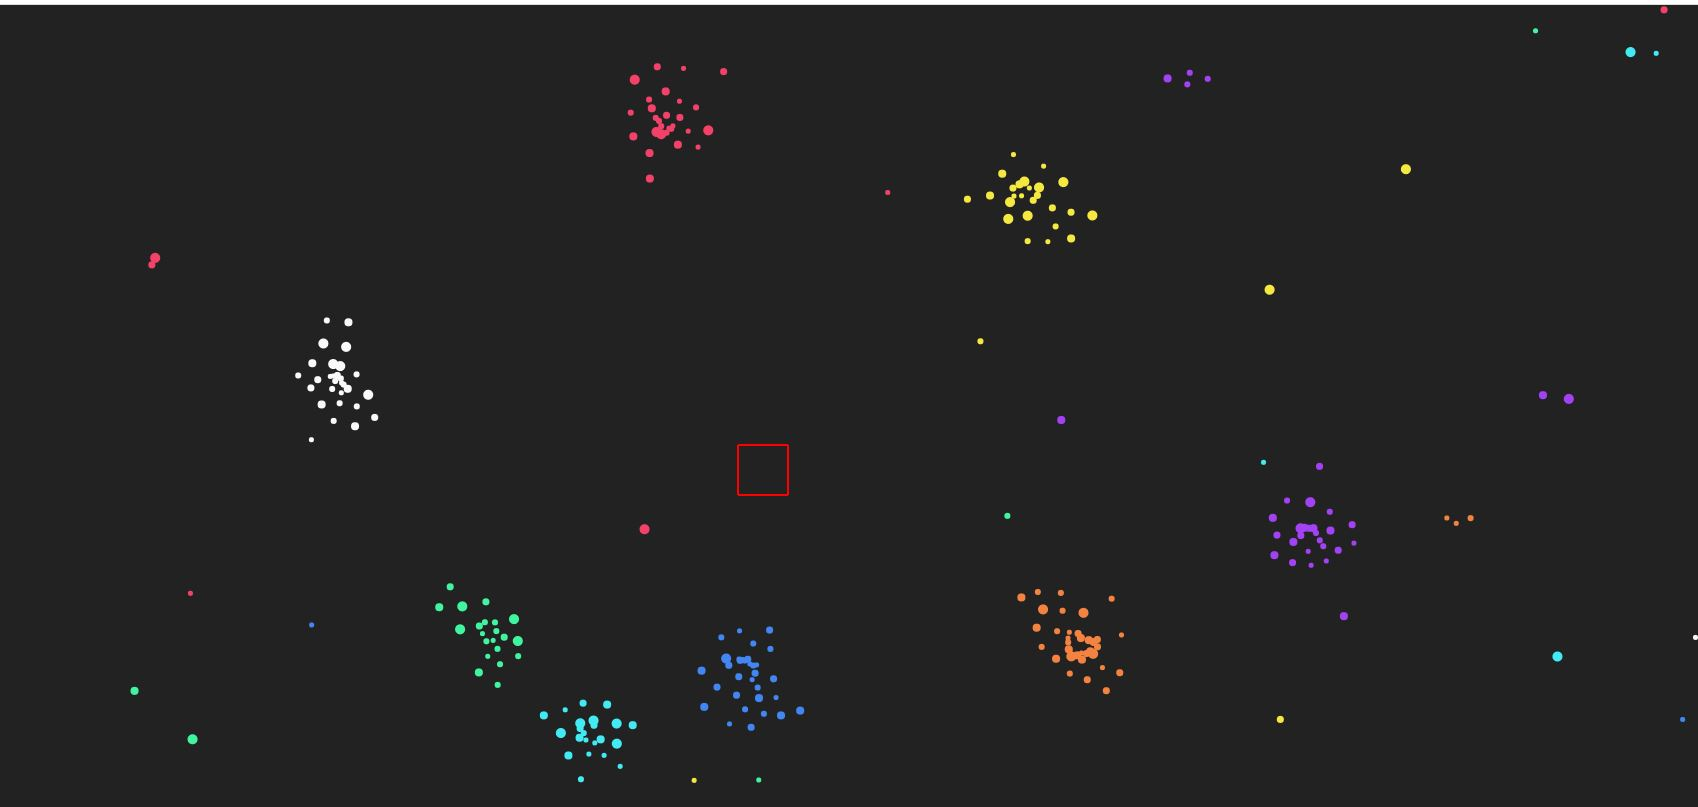
\includegraphics[scale=0.4]{gambar/example}
% \caption{Hasil Model alligment,separation dan kohesi}
% \end{figure}
% \hspace{0.6cm}
\begin{figure}
\centering
\subfigure[Model Flocking dengan range 25 N=100]{\label{fig:flocking dengan range 25}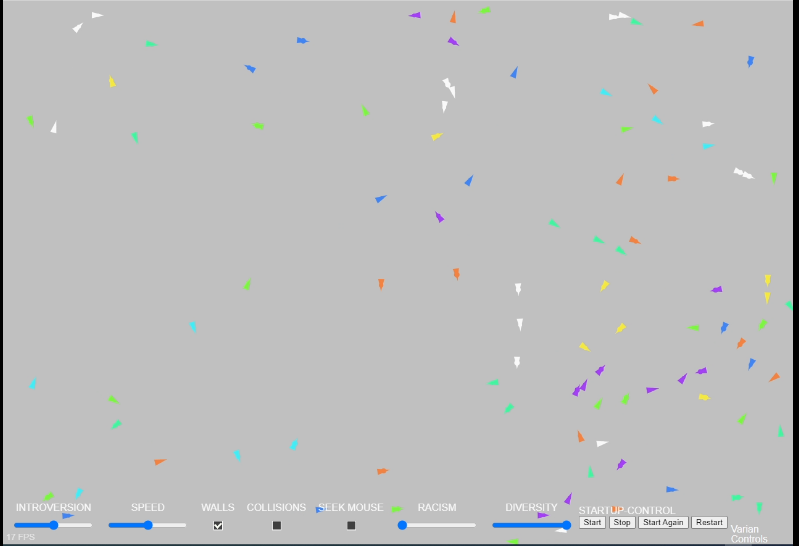
\includegraphics[scale=0.3]{gambar/gambar1notawafflocking25}}
\hfill
\subfigure[Grafik Model Flocking dengan range 25 N=100]{\label{fig:grafik flocking dengan range 25}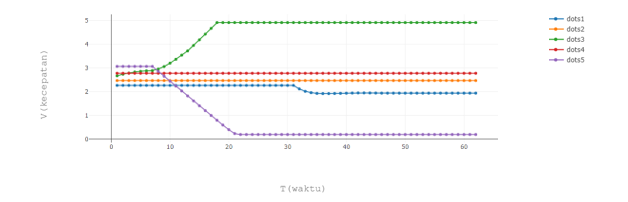
\includegraphics[scale=0.45]{gambar/datagrafik/range25homogennoflocking}}

\subfigure[Model Flocking dengan range 50 N=100]{\label{fig:flocking dengan range 50}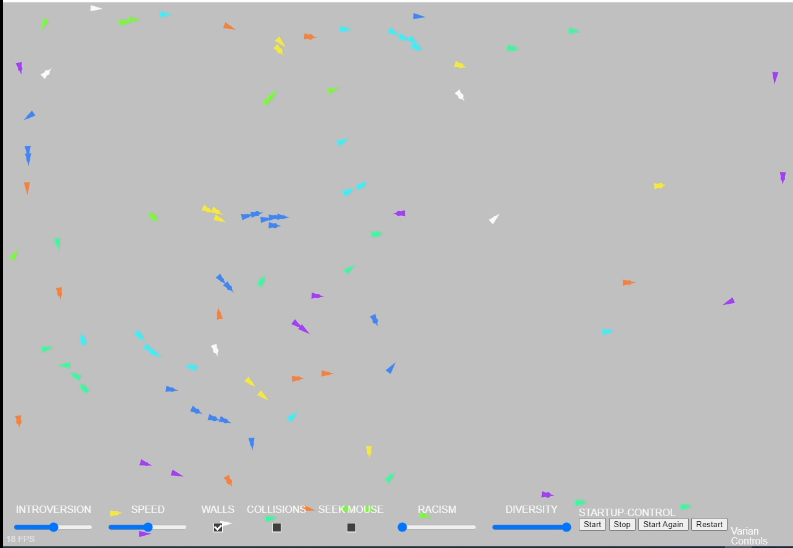
\includegraphics[scale=0.3]{gambar/gambar2notawafflocking50}}
\hfill
\subfigure[Grafik Model Flocking dengan range 50 N=100]{\label{fig:grafik flocking dengan range 50}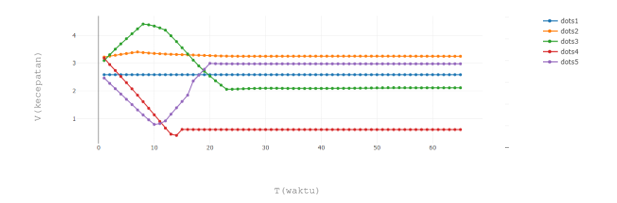
\includegraphics[scale=0.45]{gambar/datagrafik/range50noflocking}}

\caption{Hasil Model alligment,separation dan kohesi dengan range 25 dan range 50}
\label{fig:2grafikmodel3gaya}
\end{figure}

% Pada hasil ini formasi partikel terlihat bisa membedakan partikel hal ini karena 
Hasil pada model \textit{flocking} tanpa gerakan tawaf(\textit{circular motion}) dengan \textit{range} \textit{flocking} yang berbeda pada kohesi dan pensejajarannnya, dapat dibandingkan kedua pengoptimalan \textit{range} dalam menentukan pergerakan partikel . Hal ini dapat dibandingkan dengan \citep{HUTH1992} juga yang membuat \textit{range}, agar perbedaan pergerakan partikel dapat terlihat.Pada gambar \ref{fig:2grafikmodel3gaya} partikel yang mempunyai \textit{range} 50 cenderung lebih mudah berkelompok  dari pada \textit{range} 25. hal ini wajar karena semakin besar \textit{range} dalam \textit{flocking} yang digunakan maka semakin mudah dalam partikel berkelompok. Pada partikel dengan \textit{range} 50 berkelompok adalah 4 partikel sedangkan pada partikel dengan \textit{range} 25 berkelompok adalah 2 partikel. 

\hspace{0.6cm} Pada grafik \ref{fig:grafik flocking dengan range 25} partikel mulai dari kecepatan yang berbeda-beda sampai kecepatan tetap pada iterasi ke 10. Dan grafik\ref{fig:grafik flocking dengan range 50} sampai kecepatan tetap pada iterasi ke 20. Hal ini sesuai dengan kaidah \textit{flocking} pada \citep{Bajec2007} 
% \hspace{0.6cm}Hasil sementara berupa gerak flocking yaitu allignment, separation dan kohesion yang dipadukan dengan fungsi mencari titik pusat. Metode yang digunakan masih euler karena memperhitungkan buffer yang terjadi jika memakai runge kutta.  Koeffisien separation divariasikan dengan racism dan introversion agar terlihat jamaah mempunyai identitas yang berbeda. Pembentukan formasi berdasarkan warna partikel dimana partikel mampu membedakan satu sama lain 

%%%%%%%%%%%%%%%%%%%%%%%%%%%%%%%%%%%%%%%%%%%%%%%%
\section{Flocking dengan Gaya Dominan(Circular Motion)}%\label{sec:alat}

\begin{figure}
\centering

\subfigure[Hasil Model dengan ditambahkan gaya dominan, N=100]{\label{fig:2grafikmodel4gayadengan dominanforce}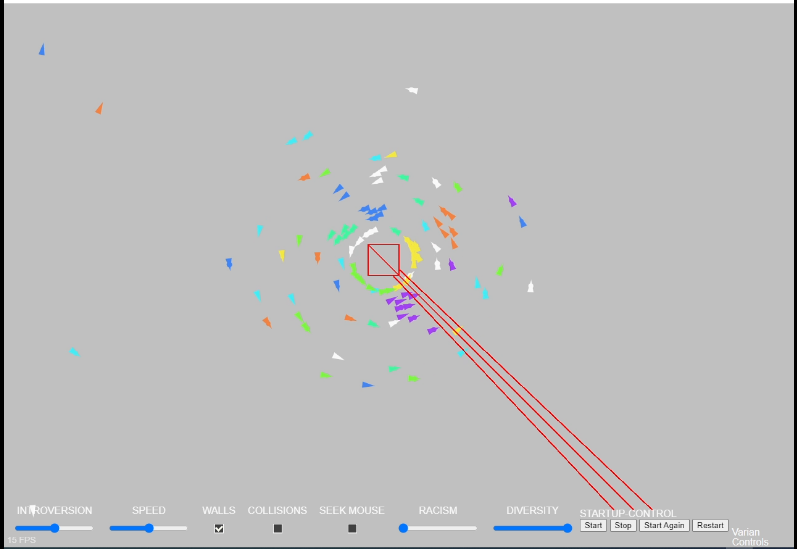
\includegraphics[scale=0.6]{gambar/gambar3tawafflocking25}}

\hfill
\subfigure[Grafik Model Flocking dengan gaya dominan, range 25 N=100]{\label{fig:grafik flocking dengan gaya dominan range 25}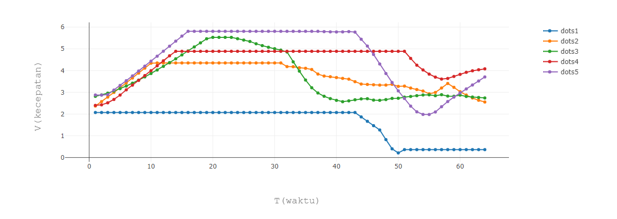
\includegraphics[scale=0.45]{gambar/datagrafik/range25homogen}}
\hfill
\subfigure[Grafik Model Flocking dengan gaya dominan range 50 N=100]{\label{fig:grafik flocking dengan gaya dominan range 50}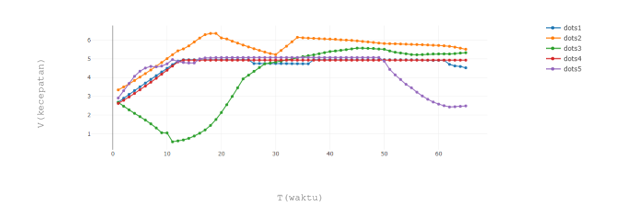
\includegraphics[scale=0.45]{gambar/datagrafik/range50homogen}}
\end{figure}
\hspace{0.6cm} Pada bagian ini ditambahkannya gaya dominan pada persamaan 2.5 dimana gaya dominan ini berfungsi mengikat partikel untuk berputar pada porosnya.Terdapat perbedaan antara pergerakan tanpa circular motion adalah \textit{flocking} hanya bekerja pada area tawaf. Dan partikel diluar area tersebut akan perlahan mendekati area tawaf. Hal ini dilakukan untuk mendekati \citep{Nasir2016} dan \citep{Kim2014}. Dimana apa yang dilakukan nasir adalah mengelompokan partikel dalam sebuah group dikelilingi partikel yang homogen. sedangkan pada \citep{Kim2014} mengamplikasikan \textit{flocking} ditambahkan dengan reciprocal coalition avoidance. untuk memperlihatkan interaksi partikel yang lebih tidak bersinggungan. Jika dapat dianalisis hasil pada \ref{fig:2grafikmodel4gayadengan dominanforce} didapat konsep \citep{Nasir2016} yang menggolongkan partikel dan konsep dari \citep{Kim2014} untuk \textit{flocking} berbasis kecepatan.

\hspace{0.6cm}Pada kedua grafik, model \textit{flocking} dengan gaya dominan \ref{fig:grafik flocking dengan gaya dominan range 25},\ref{fig:grafik flocking dengan gaya dominan range 50} menggunakan 2 variabel \textit{range} yang berbeda yaitu 25 dan 50. Kedua grafik jika dibandingkan dengan hasil grafik awal tidak mencapai keadaan \textit{flocking}. Hal ini dipengaruhi oleh gaya dominan, untuk mencapai \textit{flocking} yang linier maka dilakukan simulasi kembali pada bagian bab selanjutnya. 

\section{Flocking dengan Gaya Dominan(Circular Motion) partikel dengan Karakteristik}%\label{sec:alat}

% \begin{figure}
% \centering
% \includegraphics[scale=0.4]{gambar/}
% \caption{Hasil Model Sementara}
% \end{figure}
\begin{figure}
\centering
\subfigure[Model Flocking dengan range 25 N=100 gaya dominan tawaf]{\label{fig:flocking dengan range 25 dominan force}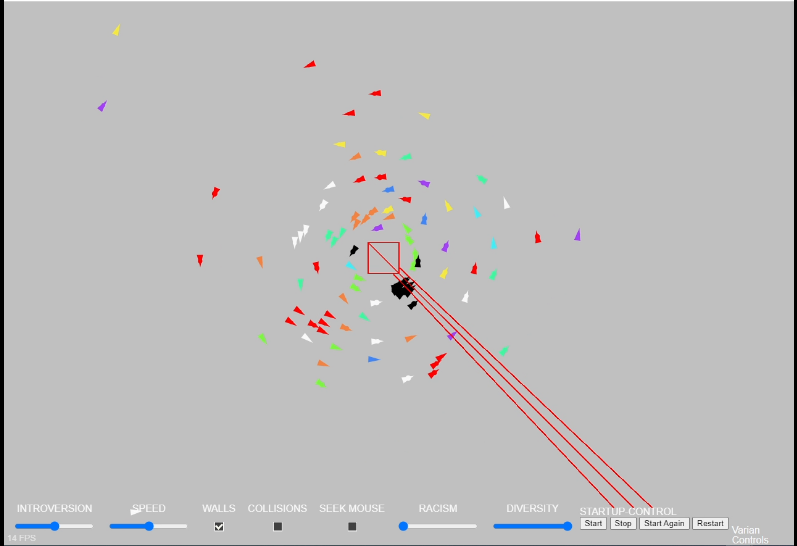
\includegraphics[scale=0.4]{gambar/gambar4tawafflocking25variabel}}
\hfill
\subfigure[Grafik Model Flocking dengan range 25 N=100 gaya dominan tawaf]{\label{fig:flocking dengan range 25 dominan force}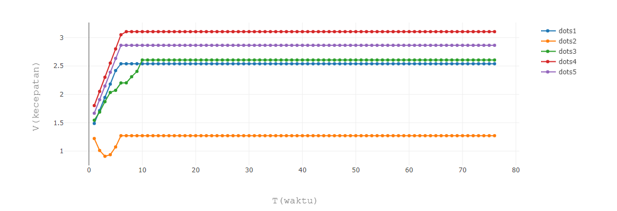
\includegraphics[scale=0.45]{gambar/datagrafik/range25heterogen}}


\subfigure[Model Flocking dengan range 50 N=100 gaya dominan tawaf]{\label{fig:flocking dengan range 50 dominan force}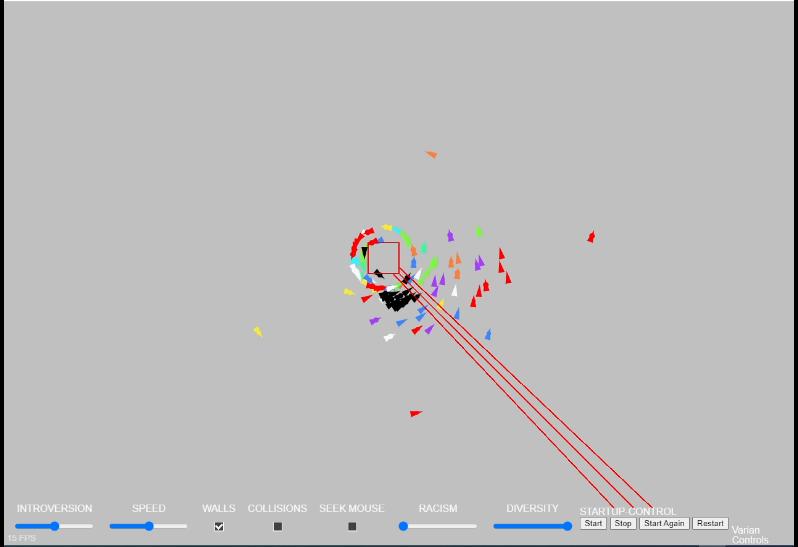
\includegraphics[scale=0.4]{gambar/gambar5tawafflocking50variabel}}
\hfill
\subfigure[Grafik Model Flocking dengan range 50 N=100 gaya dominan tawaf]{\label{fig:flocking dengan range 50 dominan force}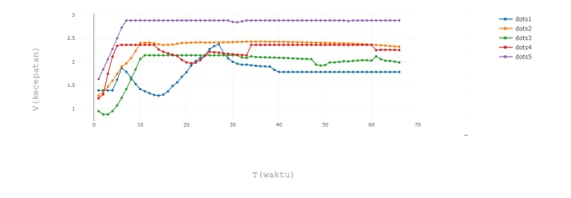
\includegraphics[scale=0.45]{gambar/datagrafik/range50heterogen}}

\caption{Hasil Model alligment,separation dan kohesi dengan range 25 dan range 50 ditambah dengan dominan force tawaf}
\label{fig:2grafikmodel4gaya}
\end{figure}

Dan terakhir pada bagian ini kami menambahkan 2 jenis partikel dengan kecepatan yang berbeda di kedua sistem \textit{range} yang berbeda. Disini dapat terlihat pada gambar \ref{fig:2grafikmodel4gaya} (kanan) ternyata \textit{range} yang lebih besar mendistrupsi sistem \textit{flocking} pada gerakan tawaf. Hal ini dapat terlihat dari partikel yang tertarik menuju pusat. Hasil yang berbeda didapat dari sistem yang menggunakan \textit{range} lebih kecil \ref{fig:2grafikmodel4gaya}(kiri). Partikel cenderung melakukan menyebar dalam area tawaf dan melakukan \textit{flocking} dengan lebih optimal. 

Penambahan variabel dari kecepatan partikel ini (merah dengan 1.25 kecepatan partikel biasa) dan (hitam dengan 0.75 partikel biasa). dapat memperlihatkan pada bagian optimal gambar  \ref{fig:2grafikmodel4gaya}(kiri). Bahwa partikel hitam cenderung bergerak di pusat sedangkan partikel merah berada di luar. Hal ini disebabkan karena gaya dominan melebihi gerak \textit{flocking}.

\hspace{0.6cm}Sedangkan dengan sudut pandang grafik, pada grafik \ref{fig:flocking dengan range 25 dominan force} kecepatan tetap pada titik tertentu dibandingkan grafik \ref{fig:flocking dengan range 50 dominan force}. Hal ini karena variasi penulis untuk mendapatkan hasil yang linier mengikuti kaidah \textit{flocking} bahwa kecepatan partikel akan tetap pada titik tertentu seperti dalam \citep{Bajec2007}. Gaya dominan seperti pada grafik \ref{fig:grafik flocking dengan gaya dominan range 25},\ref{fig:grafik flocking dengan gaya dominan range 50} tidak mengganggu dengan hasil \ref{fig:flocking dengan range 25 dominan force}
% \begin{figure}
%      \centering
%      \begin{subfigure}[b]{0.03\textwidth}
%          \centering
%          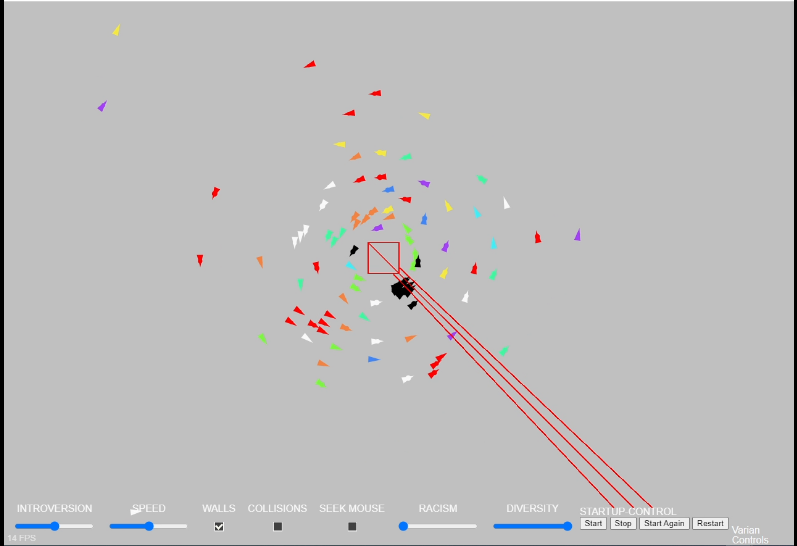
\includegraphics[width=\textwidth]{gambar/gambar4tawafflocking25variabel}
%          \caption{Model Flocking dengan range 25 N=100 Dominan force tawaf}
%          \label{fig:flocking dengan range 25 dominan force}
%      \end{subfigure}
%      \hfill
%      \begin{subfigure}[b]{0.03\textwidth}
%          \centering
%          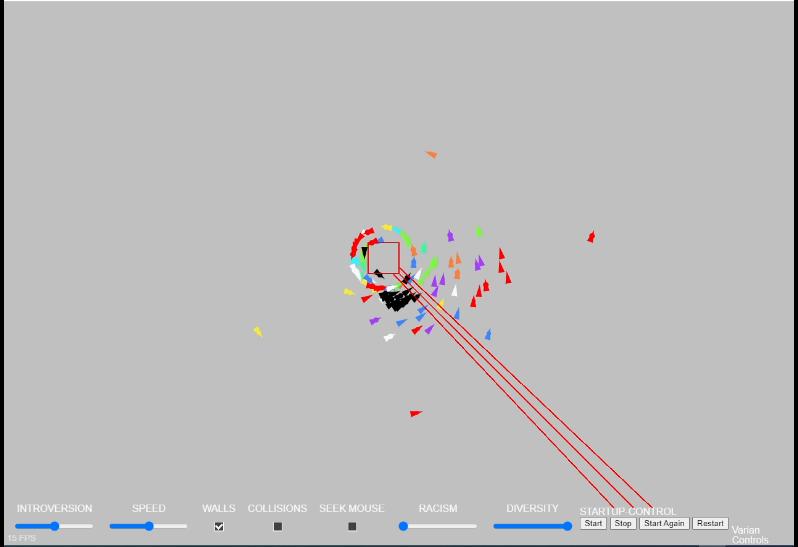
\includegraphics[width=\textwidth]{gambar/gambar5tawafflocking50variabel}
%          \caption{Model Flocking dengan range 50 N=100 Dominan force tawaf}
%          \label{fig:flocking dengan range 50 dominan force}
%      \end{subfigure}
%         \caption{Hasil Model alligment,separation dan kohesi dengan range 25 dan range 50 ditambah dengan dominan force tawaf}
%         \label{fig:2 grafik model 4 gaya}
% \end{figure}
%%%%%%%%%%%%%%%%%%%%%%%%%%%%%%%%%%%%%%%%%%%%%%%%

% \subsection{Optimasi circular  motion dengan partikel Karakteristik}
% \begin{figure}
% \centering
% 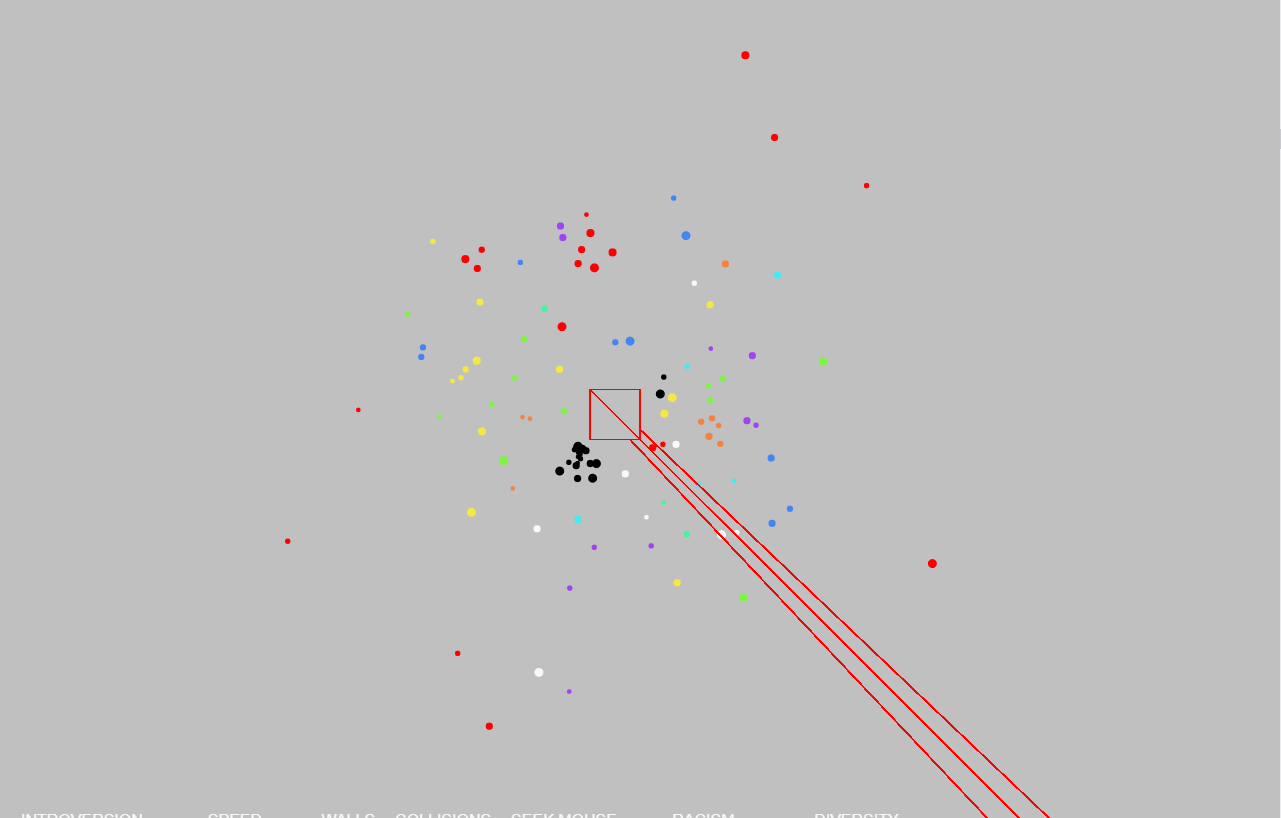
\includegraphics[scale=0.4]{gambar/speed1.5dan0.75.PNG}
% \caption{Hasil Model dengan partikel speed 1.5(merah) dan partikel speed 0.75(hitam)  }
% \end{figure}
% \hspace{0.6cm}Pada Flocking 
%%%%%%%%%%%%%%%%%%%%%%%%%%%%%%%%%%%%%%%%%%%%%%%
\section{Perbandingan Hasil Simulasi dengan Beberapa Referensi}
\subsection{Referensi Hasil Simulasi dengan \citep{Kim2014} }%\label{sec:alat}
\begin{figure}
\centering
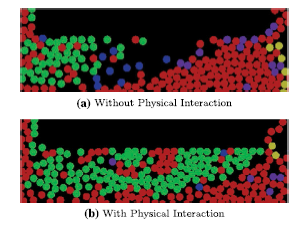
\includegraphics[scale=0.6]{gambar/Kim2014}
\caption{Hasil Gerak Partikel pada \citep{Kim2014}}
\label{fig:figkim2014}
\end{figure}

\hspace{0.6cm} Pada gambar \ref{fig:figkim2014} diperlihatkan hasil kim bahwa partikel (agen) terpadatkan di dekat pusat area gaya(kaaba). Hal ini dikarenakan terdorong oleh kerumunan agen. Pada gambar agen hijau menunjukan agen yang menunggu menyentuh titik pusat gaya(hajar aswad). Diawal simulasi agent berada dalam keadaan tidak dapat bergerak dan menghasilkan kerumunan padat. Tanpa interaksi fisis meskipun ada ruang gerak, partikel agent tidak bisa memproses ke posisi selanjutnya. Dengan tambahan interaksi fisis dengan agent selanjutnya agent dapat terdorong oleh kerumunan.
% \hspace{0.6cm}Dapat terlihat bentuk tawaf telah terbentuk, mungkin harus ada adjustment gaya lagi supaya geraknya selalu melawan arah jarum jam. Boundary state untuk partikel juga belum diterapkan seperti dinding kaaba dan outer dinding bagian masjid, kemunculan partikel sendiri harus ada adjustment. dan harus ada adjustment lagi tentang layar yang digunakan untuk menetukan kecepatan yang terbentuk.
%%%%%%%%%%%%%%%%%%%%%%%%%%%%%%%%%%%%%%%%%%%%%%%%
\subsection{Referensi Hasil Simulasi dengan \citep{Nasir2016}}%\label{sec:alat}
\begin{figure}
\centering
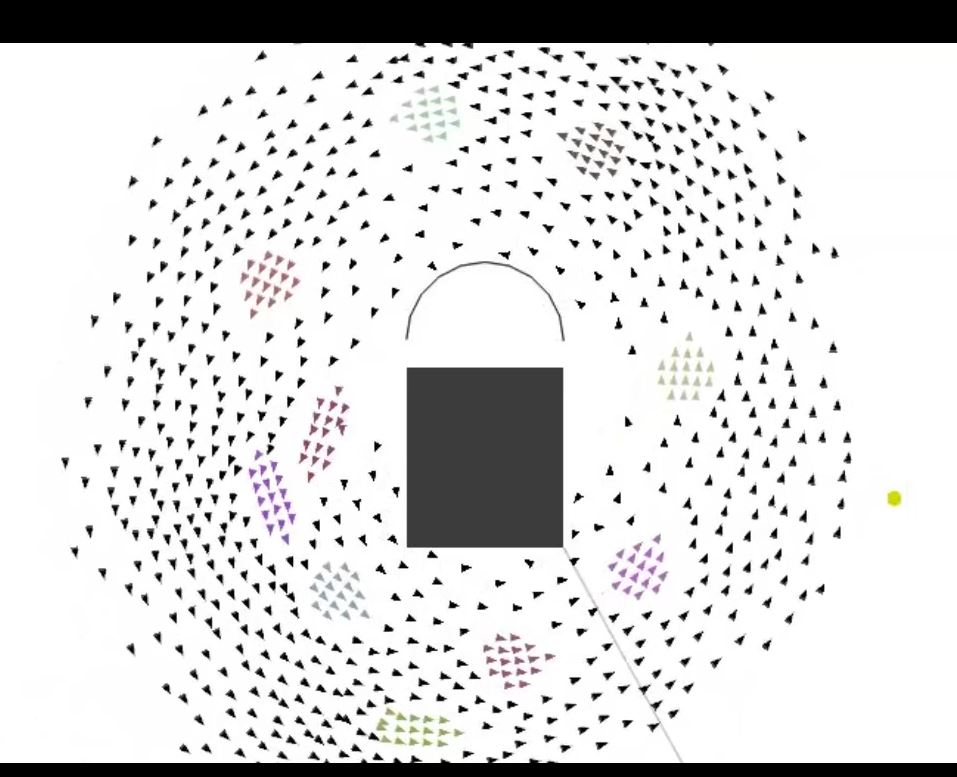
\includegraphics[scale=0.4]{gambar/PaperNasir.JPG}
\caption{Hasil model oleh Nasir}
\label{fig:nasir1}
\end{figure}
\hspace{0.6cm}Bentuk model tawaf dari nasir\citep{Nasir2016} ditunjukan pada gambar diatas. Perilaku partikel berkelompok pada nasir memiliki kecepatan yang sama atau tidak lebih cepat dari partikel sekitarnya. Hal ini yang membuat formasi lebih solid, jika dibandingkan.

\hspace{0.6cm} Hasil penelitian yang telah dilakukan oleh \citep{Nasir2016} ditunjukan oleh \ref{fig:nasir1}. Lingkungan yang dimiliki partikel diletakan kabah berbentuk persegi bersama dengan area bidang perisai untuk hijir ismail. Partikel bergerak berkelompok bersama dengan partikel sejenis dan membuat gerakan tawaf. Hal ini jika dibandingkan dengan dengan hasil pada \ref{fig:2grafikmodel4gaya}(kiri) terdapat banyak perbedaan, diantaranya pergerakan partikel yang cenderung lebih mendekati pusat gaya(kaaba) dan kelompok lebih dapat terpencar, kemudian membuat kelompok yang lebih kecil lagi.

\subsection{Referensi Hasil Simulasi dengan \citep{Bajec2007}}%\label{sec:alat}
\begin{figure}
\centering
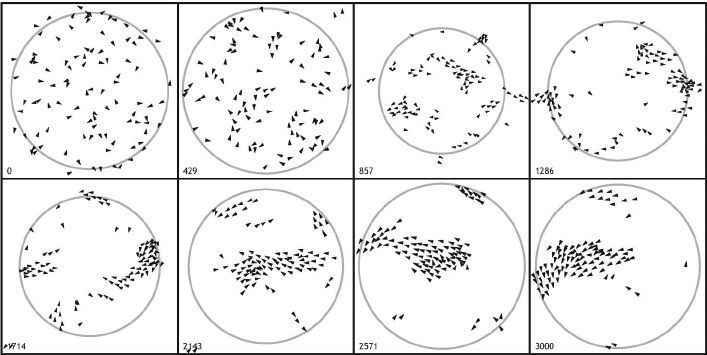
\includegraphics[scale=0.4]{gambar/Bajec.PNG}
\caption{Hasil Flocking Bajec}
\label{fig:bajec1}
\end{figure}
\hspace{0.6cm}Hasil penelitian yang telah dilakukan oleh \citep{Bajec2007} ditunjukan oleh \ref{fig:bajec1}. Area bergerak yang dimiliki partikel berbentuk lingkaran, Ketika partikel melewati batas tersebut maka akan ada gaya yang memaksanya bergerak kembali ke dalam. Jika dibandingkan antara hasil pada Gambar \ref{fig:2grafikmodel3gaya}  dengan Gambar \ref{fig:bajec1}, maka tidak jauh berbeda. Hal ini terlihat dari pola gerak partikel yang pada awalnya tidak berkelompok kemudian menjadi berkelompok dengan beberapa kelompok kecil dan satu kelompok terbesar. 



%\input{referensi}
%\end{document}

\subsection{Referensi Hasil Simulasi dengan \citep{Nasir2016}}%\label{sec:alat}